% !TeX root = ../../tfg.tex
% !TeX encoding = utf8
%
%***************************************************************
% Contenido del artículo 5: Generalización a multi-output 
%***************************************************************
\section{Generalización para \textit{multi-output neuronal networks}}

En las secciones anteriores se han provisto resultados para redes 
neuronales de salida real. Vamos a generalizar los resultados vistos
para ser capaces de aproximar funciones continuas o medibles 
de $\R^r$ a $\R^s$ con $r,s \in \N.$

Denotaremos como $\fCC$ al conjunto de funciones continuas definidas de $\R^r$ a $\R^s$ y al de funciones medibles de 
$\R^r$ a $\R^s$  como $\fMM.$ 
La distancia asociada a estos espacios se define como 
\begin{equation}
    \rho_{\mu}^s(f,g) 
    =
    \sum_{i=1}^s \dist(f_i, g_i).
\end{equation}

\text{red}{Falta afinar estas definiciones}

Con la siguiente definición buscamos abstraer el modelo de una red neuronal de una capa oculta y salida múltiple.
\begin{figure}[h]
    \centering
    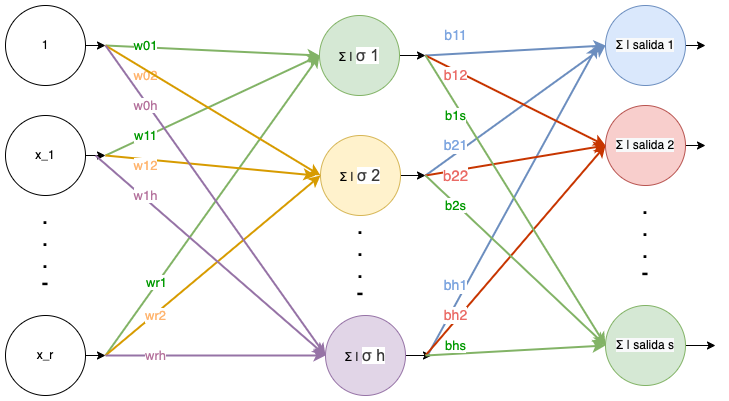
\includegraphics[width=.7\textwidth]{articulo_rrnn_aproximadores_universales/RedNeuronalAbstactaUnaCapaVariasSalidas.png}
    \caption{Ejemplo de red neuronal de una capa oculta con $h$ nodos, de dimensión de entrada $r$ y salida $s$.}
    \label{fig:red neuronal-r-h-s}
\end{figure}

Nótese que los vectores $(w_{0i},w_{1i}, \ldots, w_{ri})$ representan a la aplicación afín 
$A_i((x_1, x_2, \ldots x_r)) = w_{0i} + \sum_{j=1}^r w_{ji} x_j$
con $i \in \{1,\ldots, h\}$ . 

\begin{definicion}[Abstracción red neuronal una capa oculta múltiple salida] 
    Para cualquier función Borel medible $G$, definida de $\R$ a $\R$ y cualquier natural positivo
    $r \in \N$ se define a la clase de funciones $\pmc$ como 
    \begin{equation}
        \begin{split}
        \sum^{r,s}(G) = 
        \{ 
            & f: \R ^r \longrightarrow \R^s, f= (f_1, f_2, \ldots f_s)  / \quad 
            \\ &
            \text{ con } f_i : \R ^r\longrightarrow \R, 
            f_i(x)=\sum_{j = 1} ^h (
            \beta_{j i} G(A_{j}(x)) \quad i \in \{1,2,\ldots, s\}, \\
            & x  \in \R ^r, \beta_{j i} \in \R, A_{j}\in A^r,h \in \N
            )
        \}.
        \end{split}
    \end{equation}
\end{definicion}
y no es difícil pensar que su versión generalizada sea: 

\begin{definicion} 
    Dadas las mismas hipótesis que en la definición anterior, se define la siguiente clase de funciones como 
    \begin{equation}
        \begin{split}
            \sum \prod^{r, s}(G) 
            = 
        \{ 
            & f: \R ^r \longrightarrow \R^s, f= (f_1, f_2, \ldots f_s)  / \quad 
            \\ &
            \text{ con } f_i : \R ^r\longrightarrow \R, 
            f_i(x)=\sum_{j = 1} ^h 
            \left(
            \beta_{j i} \prod_{k=1}^{l_{j i}} G(A_{j i}(x)
            \right)
             \quad i \in \{1,2,\ldots, s\}, \\
            & x  \in \R ^r, \beta_{j i} \in \R, A_{j i}\in A^r; h,l_{j i} \in \N
            )
        \}.
        \end{split}
    \end{equation}
\end{definicion}

% Corolario 2.6  
\begin{corolario}\label{corolario:2_6}
    Los teoremas 
    \ref{teorema:2_3_uniformemente_denso_compactos}
    \ref{teo:2_4_rrnn_densas_M} 
    y los corolarios
    \ref{cor:2_1}, 
    \ref{corolario:2_2_rrnn},
    \ref{corolario:2_3_medida_probabilidad},
    \ref{corolario:2_4_conjunto_finito}
    y 
    \ref{corolario:2_5_función_Booleana}
    permanecen válidos si se sustituye $\rrnn$ por $\rrnnmc$
    ,$\rrnng$ por $\rrnngmc$, 
    los espacios de funciones continuas y medibles por $\fCC$ y $\fMM$ respectivamente con su respectiva norma.
\end{corolario}
\begin{proof}
    \textcolor{red}{TODO}
\end{proof}

% Lema A.6   
\textcolor{red}{La demostración expuesta en el artículo de este lema es incorrecta, ya que en él se afirma que 
si $|f(x) - x| <= e$ entonces $|g(f(x))- g(x)|$ es menor $e$. Esto claramente es un error ya que 
consideremos $g(x) = 2x$ y $f(x)=x+e$, está claro que $|g(f(x))- g(x)|=2e>e$. Es por ello que propongo esta
demostración alternativa basada en el conjunto $\Lambda_{K, \delta, g}$.}
\begin{lema}
    Sea F un conjunto de funciones definidas de $\R \longrightarrow \R$ que es uniformemente 
    denso para compactos de $C(\R)$ y
    G un conjunto de funciones definidas de $\R^r \longrightarrow \R$ que es uniformemente 
    denso para compactos de $\fC$.
    
    Se tiene entonces que el conjunto 
    \begin{equation}
        G \circ F 
        = 
        \{
            g \circ f : g \in G \text{ y } f \in F
        \}
    \end{equation}
    es uniformemente denso para compactos de $\fC.$
\end{lema}
\begin{proof}
    Queremos probar que para cualquier $h \in \fC$, cualquier conjunto compacto $K \subset \R^r$ 
    y cualquier $\epsilon >0$
    existe una función $g \circ f \in G \circ F$ tal que 
    \begin{equation}
        \sup_{x \in K}|h(x) - g \circ f(x)| < \epsilon.
    \end{equation}

    Por ser $G$ uniformemente denso existe $g \in G$ satisfaciendo 
    \begin{equation}
        \sup_{x \in K}|h(x) - g(x)| < \frac{\epsilon}{2}.
    \end{equation}
    Definimos el conjunto 
    \begin{equation}
        \Lambda_{K, \delta, g} 
        = 
        \{
           \sup|g(x) - g(s)| : x \in K, s \in \bar{B}(x,\delta) \cap K 
        \}
    \end{equation}
    Notemos que por estar en un compacto $\sup|g(x) - g(s)|$ está bien definido 
    y existe el supremo de $\Lambda_{K, \delta, g};$ además, fijando $g$ y $K$ por continuidad de $g$
    y estar en un compacto podemos encontrar un $\delta'$ tal que 
    \begin{equation}\label{lema_A_6:supremo_lambda_delta_prima}
        \sup \Lambda_{K, \delta', g}  < \frac{\epsilon}{2}.
    \end{equation}
    Por ser $F$ uniformemente denso existe $f \in F$ satisfaciendo 
    que 
    \begin{equation}\label{lema_A_6:encontramos_f}
        \sup_{x \in K}|f(x) - x| < \delta'.
    \end{equation}
    Gracias a \refeq{lema_A_6:supremo_lambda_delta_prima} y \refeq{lema_A_6:encontramos_f} se tiene que
    \begin{equation}
        \sup_{x \in K}|g \circ f(x) - g(x)| 
        < \sup \Lambda_{K, \delta', g} 
        < \frac{\epsilon}{2}
    \end{equation}
    Por lo que acabamos de probar lo buscado 
    \begin{align}
        \sup_{x \in K}|h(x) - g \circ f(x)| &
        < 
        \sup_{x \in K}|h(x) - g(x) + g(x) - g \circ f(x)| 
        \\ &
        < 
        \sup_{x \in K}|h(x) - g(x)|
        + 
        \sup_{x \in K}|g(x) - g \circ f(x)|  
        \\ &
        < 
        \frac{\epsilon}{2} + \frac{\epsilon}{2}
        = \epsilon.
    \end{align}
\end{proof}

Finalmente vamos a probar la aproximación universal 
para redes neuronales multicapas. 
\begin{corolario}
    El teorema
    \ref{teo:2_4_rrnn_densas_M} 
    y los corolarios
    \ref{cor:2_1}, 
    \ref{corolario:2_2_rrnn},
    \ref{corolario:2_3_medida_probabilidad},
    \ref{corolario:2_4_conjunto_finito},
    \ref{corolario:2_5_función_Booleana}
    y 
    \ref{corolario:2_6}
    son válidos para 
    TODO terminar de copiar. 
\end{corolario}